\chapter{Motivation and Approach}

\section{Adaptive sampling: Motivation}
Biomolecules fulfill many different roles in nature and have accordingly a wide range of timescales associated with the conformational dynamics of the biomolecule. Molecular dynamics (MD) simulations have become indispensable for gaining
insight into the behavior of biomolecules at high spatial and temporal resolutions.
However, a fundamental limitation for MD with accurate all-atom force-fields remains
the computational demand for simulating processes with long timescales. In
particular, many biologically relevant processes, such as protein folding and
conformational changes, typically require simulation times which are orders of magnitude longer than
milliseconds. In contract, atomic-resolution MD trajectories can currently reach only timescales in the order of milliseconds. 

The ambition of this thesis is coming closer to solving the challenge of accurately determining the conformational dynamics of proteins. This challenge is immense due to the many orders of improvements necessary. Many approaches have been implemented which improve the sampling of proteins, including hardware advances and improved molecular dynamics software. Some of the approaches are introduced in this chapter. One particular approach this thesis studies is \emph{adaptive sampling}. Adaptive sampling uses many shorter MD trajectories to sample the protein energy landscape and the increased efficiency of sampling is reached by selecting the starting points of the MD trajectories based on the results of previous MD trajectories. This approach allows sampling more efficiently any high-dimensional stochastic systems. Proteins are a common example of high-dimensional stochastic systems.

\section{Outline}
 
Overall this Dissertation resulted in several peer-reviewed publications \cite{Adstrategies2018, Extasy2016}, as well one publication under review \cite{Extasy2019}. The results obtained during this Dissertation, as well as the results in the papers, will be presented in the next chapters.
 
Chapter 2 will summarize some of the standard techniques, which will be used frequently throughout the thesis. While some of these approaches are commonly used in this field, there are also recently developed techniques that are less commonly used. The relevance of all these techniques for adaptive sampling will be highlighted. 

The theory of adaptive sampling will be discussed in Chapter 3, as well the development of an upper limit of speed up with adaptive sampling will be shown. This novel result shows that adaptive sampling can be further improved. In the next chapter 4, the current strategies will be compared in a statistically robust way, and the effectiveness of each strategy will be compared for different proteins and different goals.

Chapter 5 will introduce the computational tools and software frameworks necessary to successfully and efficiently execute adaptive sampling. Due to the many subtasks adaptive sampling contains, these practical considerations have a direct impact on the viability of adaptive sampling for solving sampling problems. This software framework will be used in Chapter 6 to show the results and the accuracy which adaptive sampling can achieve for different biomolecular systems. 

A final chapter will summarize the current achievements and discuss further open questions and possible directions in further developing adaptive sampling.




\afterpage{\null\newpage}
\chapter{Background\label{sec:background}}

\section{Proteins and Molecular Dynamics}

The behavior of a protein or any biomolecule can be relatively accurately represented by Newton's classical equations of motion for atoms. All 3N atom coordinates, including the surrounding water solvent, are represented by $\mathbf{x}_{t}$ positions and $\mathbf{v}_{t}$ velocities. Figure~\ref{fig:proteins} shows the 3-dimensional structure of two of the proteins investigated in this thesis to visualize the shape of the 3D structure. The Newton's classical equations of motion are:

$$M\ddot{\mathbf{x}_{t}}=-\nabla U(\mathbf{x}_{t})$$

The potential energy $U()$ represents the all-atom force field guiding the motion of the protein. The straightforward approach of numerically solving this equation leads to a molecular dynamics (MD) trajectory describing the motion of a protein. This potential energy $U()$ approximates the quantum-mechanical dynamics of the protein and new research increasingly improves the accuracy of this approximation. An higher accuracy than all-atom folce fields would require a quantum-mechanical approach, which additionally reduces the reachable timescales by several orders of magnitude. In this thesis, the CHARMM22* force field \cite{Charmm22star} with modified TIP3P water was utilized.

\begin{figure}[H]
  \centering
  \begin{subfigure}[t]{0.45\textwidth}
    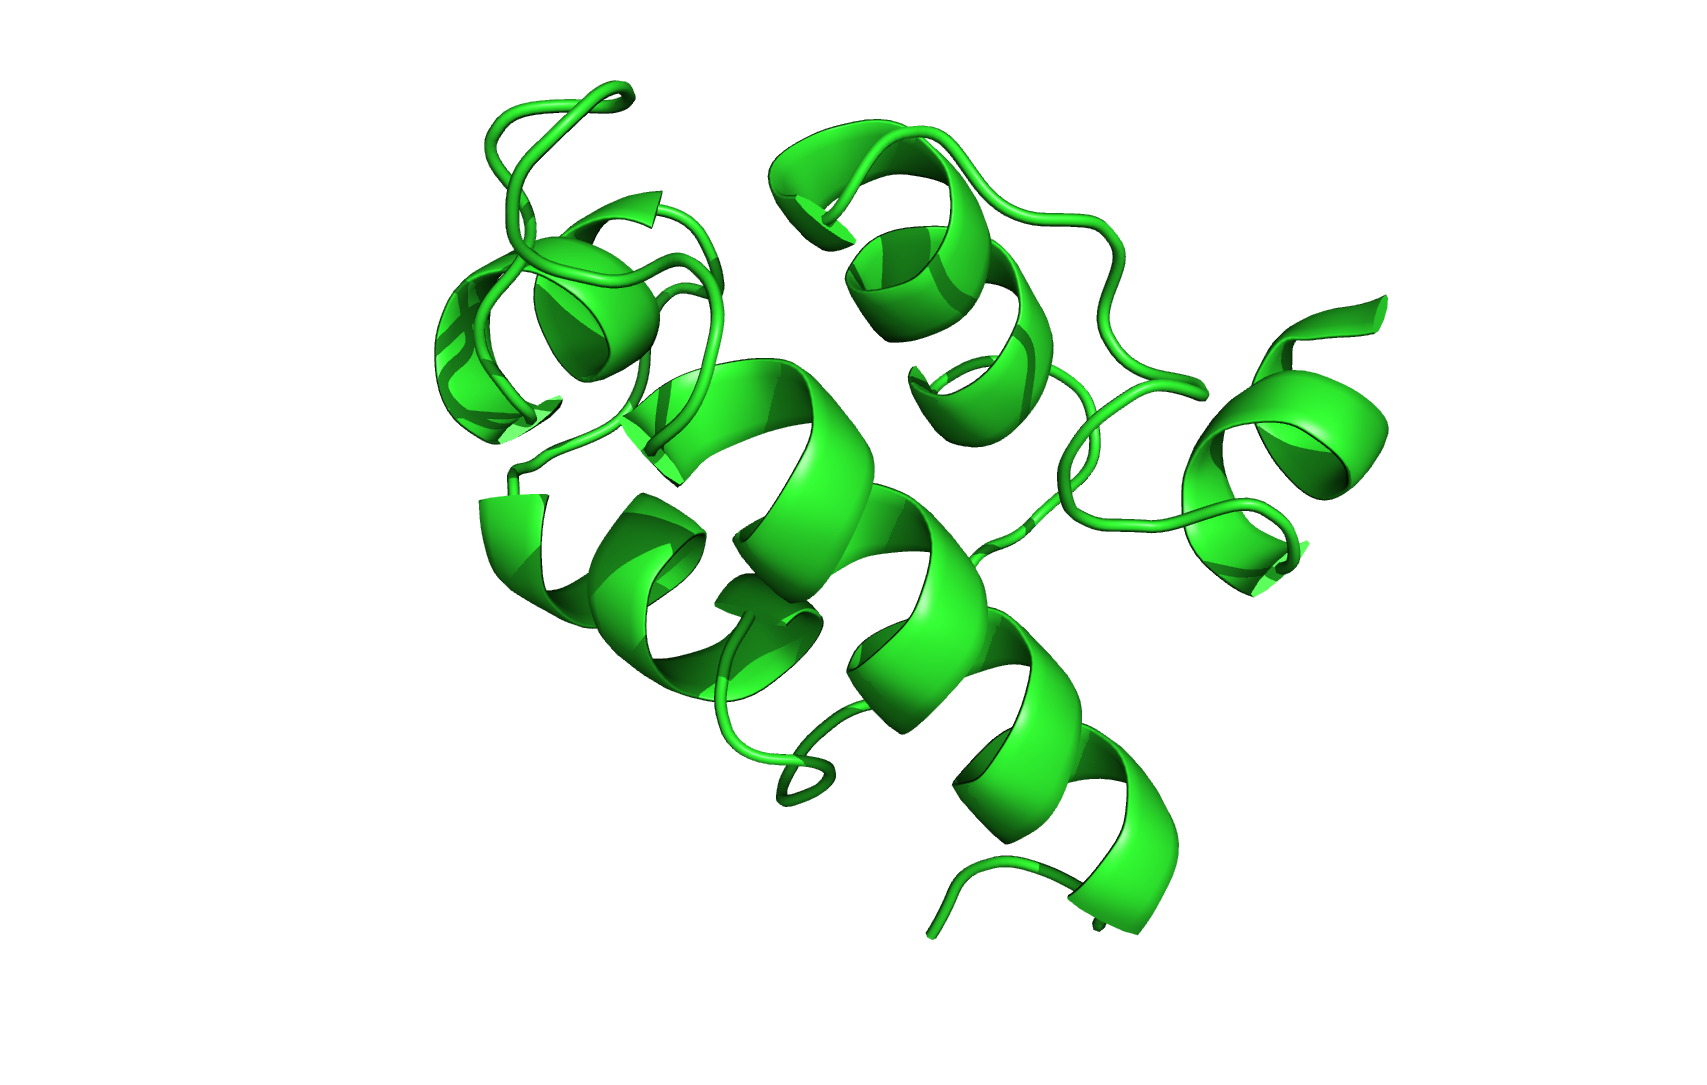
\includegraphics[width=0.9\textwidth]{figures3/lambda-repressor.png} 
  \end{subfigure}
  \begin{subfigure}[t]{0.45\textwidth}
    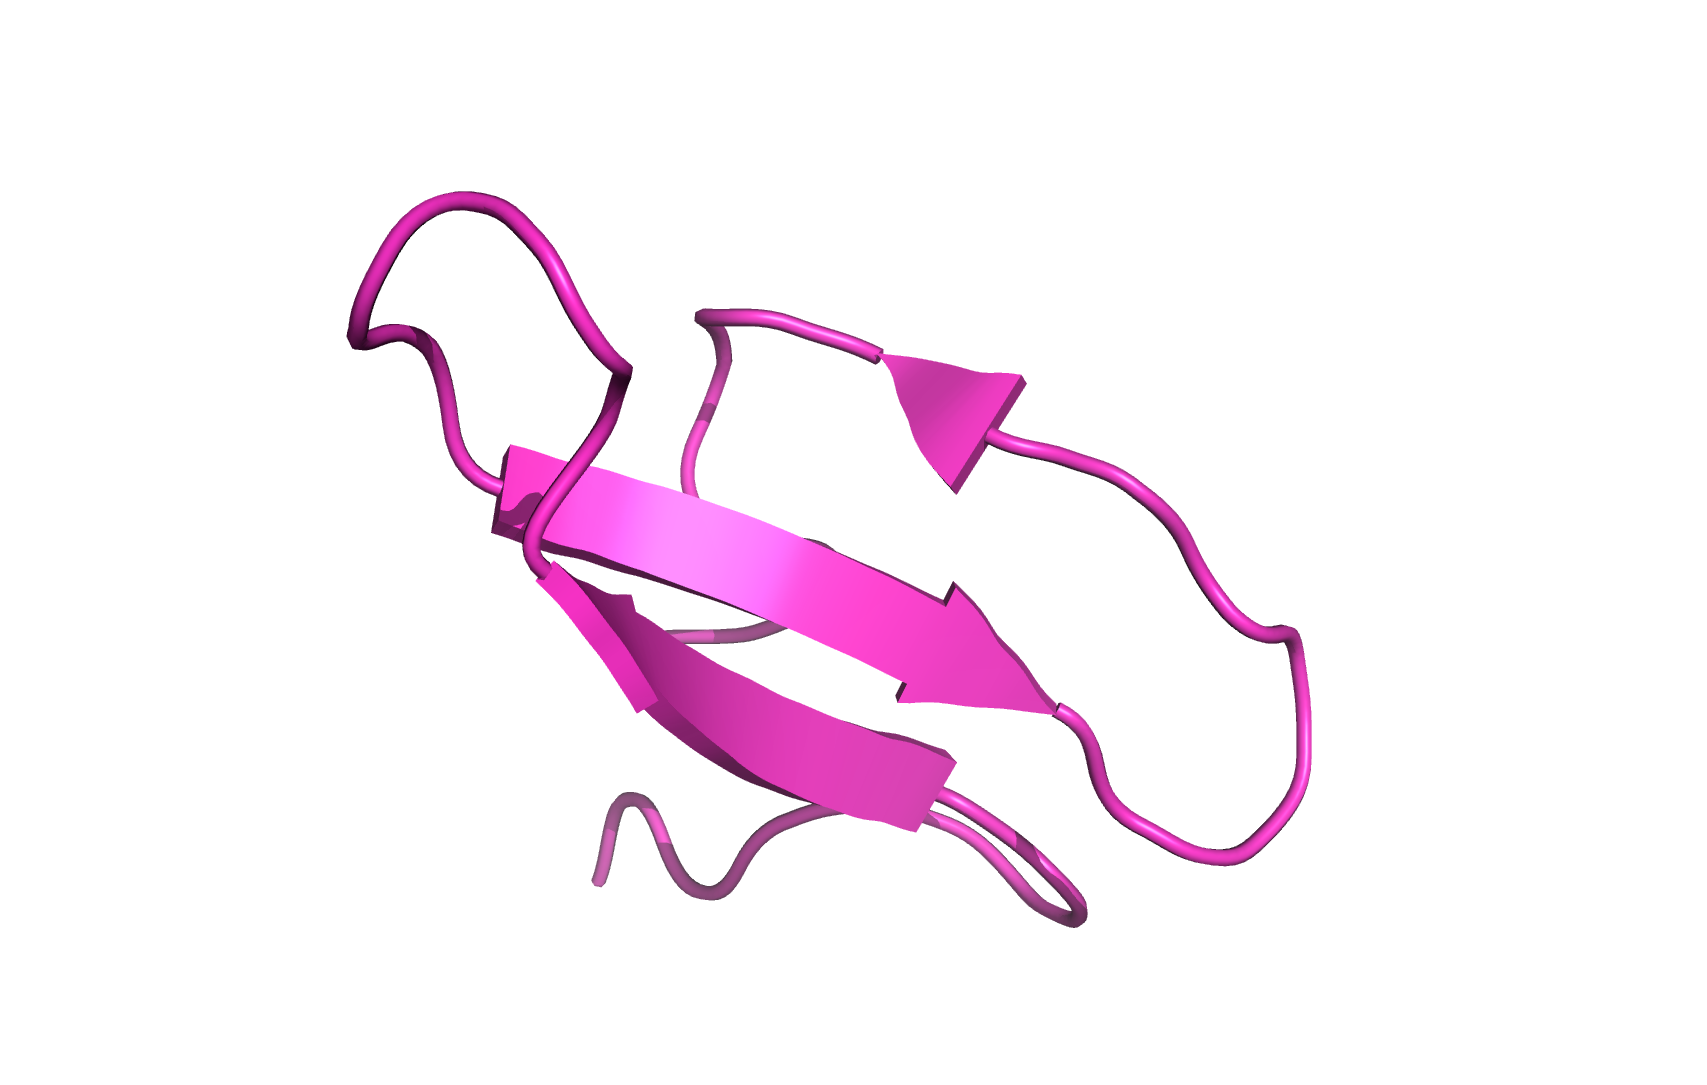
\includegraphics[width=0.9\textwidth]{figures3/ww-domain.png}  
  \end{subfigure}
  \caption{Structure of proteins $\lambda$-repressor and WW domain.}
  \label{fig:proteins}
\end{figure}


The CHARMM force field has the following potential energy, which consists of terms for molecular bonds stretching, angle bending, dihedral bending, improper dihedral energy terms, the Urey-Bradley component, non-covalent van der Waals interactions (Lennard-Jones) and Coulomb interactions. 

$$$$

\begin{equation}
\begin{aligned}
U(\mathbf{x})={}&U_{bonds}+U_{angle}+U_{dihedral}+U_{improper}+U_{UB}+U_{LJ}+U_{elec}\\
&=\sum_{bonds}K_{b}(b-b_{0})^{2}+\sum_{angles}K_{\theta}(\theta-\theta_{0})^{2}+\sum_{torsions}K_{\phi}\left(1+cos(n\phi-\delta)\right)\\
&+\sum_{impropers}k_{\omega}\left(\omega-\omega_{0}\right)^{2}+\sum_{Urey-Bradley}k_{u}\left(u-u_{0}\right)^{2}\\
&+\sum_{nonbonded}\epsilon\left[\left(\frac{R_{min,ij}}{r_{ij}}\right)^{12}-\left(\frac{R_{min,ij}}{r_{ij}}\right)^{6}\right]+\sum_{electric}\frac{q_{i}q_{j}}{\epsilon r_{ij}}
\end{aligned}
\end{equation}

In the above equation the parameters are: $k_b$ is the bond stretching force constant, $b-b_0$ is the atom distance from equilibrium, $k_\theta$ is the angle bending force constant, $\theta-\theta_0$ is the angle from the equilibrium between 3 bonded atoms, $k_\phi$ is the dihedral force constant, $n$ is the multiplicity of the dihedral function, $\phi$ is the dihedral angle, $\delta$ is the phase shift, $k_\omega$ is the improper dihedrals bending force constant, $\omega-\omega_0$ is the out of plane improper dihedrals angle, $R_{{min}_{ij}}$ is the constant for the Lennard-Jones potential, $r_{ij}$ is the distance between a pair of atoms and $q_{i}$ is the charge of an atom. The Urey-Bradley component serves the cross-term accounting for angle bending using 1,3 nonbonded interactions, where $k_{u}$ is the Urey-Bradley force constant, and $u-u_{0}$ is the distance between the 1,3 atoms in the harmonic potential.

One challenge of the straightforward approach of utilizing Newton's classical equations of motion for the prediction of protein behavior is the relatively short timestep of numerically simulating the molecular dynamics. The commonly used maximum timestep allowing for energy conservation and stability of the protein is between 2fs and 5fs. Considering most proteins fold on timescales longer than milliseconds, this requires to simulate in the order of $10^{12}$ steps. With modern GPUs, for smaller proteins, almost 1 microsecond of molecular dynamics trajectory can be simulated per day. Special purpose hardware \cite{shaw2014anton} can simulate up to 100 microseconds of MD trajectory per simulation day, but the access to this special purpose hardware is limited and commonly GPUs are used. The simulation of the behavior of most biomolecules for relevant processes such as protein folding and other global structural rearrangements requires timescales of around $10^{-2}s - 10^{0}s$. These slow processes are associated with the rare crossing of high free energy barriers, representing a bottleneck for the MD simulations.

\section{TICA dimension reduction}

A protein molecular dynamics trajectory is high-dimensional, with 1000s or more individual atom trajectories. This high-dimensionality needs to be dimension-reduced to be effectively analyzed. One approach is the Time-lagged
Independent Component Analysis (TICA) \cite{TICA1-perez2013, TICA2-schwantes2013}, which includes the kinetic information of protein dynamics in the dimension reduction.

The first step for TICA is the conversion of $\mathbf{x}_{t}$ trajectories into features $\mathbf{f}_{t}$ which are rotation- and translation-invariant and mean-free:
$$\mathbf{f}_{t}=F\left(\mathbf{x}_{t}-\left\langle \mathbf{x}_{t}\right\rangle \right)$$  
Some examples of features are atom distances or dihedral angles. The rotation- and translation-invariance is an usefull property since the protein dynamics is rotation- and translation-invariant.

The next step of TICA is the calculation of the correlation matrix $C_{00}$ and the time-lagged correlation matrix $C_{01}$:

$$C_{00}=\ensuremath{\mathbb{E}}_{t}\left[\mathbf{f}_{t}\mathbf{f}_{t}\right]$$
$$C_{01}=\ensuremath{\mathbb{E}}_{t}\left[\mathbf{f}_{t}\mathbf{f}_{t+\tau}\right]$$

The generalized eigenvalue problem for the correlation matrices leads to TICA, where $\mathbf{R}$ is the eigenvector matrix, and $\mathbf{\varLambda}$ is the diagonal eigenvalue matrix. 

$$C_{01}\mathbf{R}=C_{00}\mathbf{R}\mathbf{\varLambda}$$

The eigenvalues $\lambda_{i}$ allow the calculation of the timescales $t_{i}$. Generally, the dimensions with the longest timescales are relevant for biophysical applications.

$$t_{i}(\tau)=-\frac{\tau}{log\left|\lambda_{i}\right|}$$ 

The TICA dimension reduced trajectory $\varPsi(t)$ is obtained by projecting the feature trajectory on the $n$ slowest TICA eigenvectors. A kinetically meaningful state decomposition can be obtained with the commute map\cite{noe2016commute} where the slowest TICA coordinates are scaled with the corresponding timescales.
$$\varPsi_{commute}=\sqrt{\frac{t_{i}}{t_{o}}}\varPsi$$

The fraction of kinetic content allows the estimation of the dimensionality of the protein behavior \cite{noe2016commute}.
$$c_{m}=\frac{\sum_{i=1}^{m}t_{i}}{\sum_{i=1}^{n}t_{i}}$$

For non-equilibrium input $\mathbf{x}_{t}$ trajectories, the plain TICA will lead to inaccurate results due to the non-stationary distribution of the input correlation matrices. The Koopman method \cite{koopmanold,
koopman2,koopman3,koopman4, wu2017variational, Nueske2017} can be used to reduce
the non-equilibrium effects by reweighting the correlation matrices to the stationary distribution.

\section{State-free reversible VAMPnets}

One disadvantage of the TICA dimension reduction is the linearity of this approach. One non-linear dimension reduction is a deep learning approach with state-free reversible VAMPnets (SRV) \cite{Mardt2018,chen2019jcp}. The SRV method is closely related to the TICA methods, but with additional neuronal networks and backpropagation. The input to SRVs are the same protein trajectories $\mathbf{x}_{t}$ and feature trajectories $\mathbf{f}_{t}$ as for TICA. According to the schema in Figure~\ref{fig:NN} a neuronal network converts the input features $\mathbf{f}_{t}$ into a dimension reduced trajectory $\mathbf{o}_{t}$.

\begin{figure}[H]
  \centering
  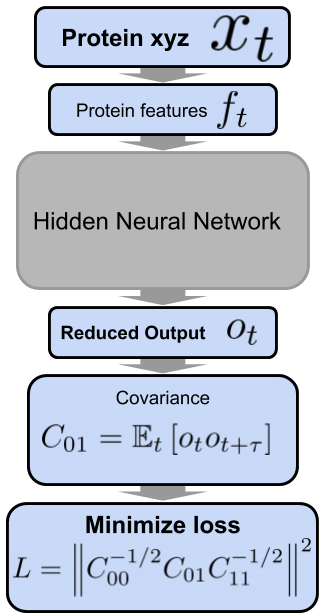
\includegraphics[width=0.4\linewidth]{figures3/NN.png}
  \caption{Schematics of the state-free reversible VAMPnets (SRV).}
  \label{fig:NN}
\end{figure}


The loss function for optimizing the parameters of the neural network with backpropagation is the VAMP-2 score:

$$L=\left\Vert C_{00}^{-1/2}C_{01}C_{11}^{-1/2}\right\Vert ^{2}$$

Here the modified covariance matrix is $C_{01}=\ensuremath{\mathbb{E}}_{t}\left[o_{t}o_{t+\tau}\right]$.
The non-linear approach of SRVs allows reaching the same accuracy as TICA for shorter lag times than TICA. TICA performs better than SRVs in the case of limited data amounts.

\section{Markov state models}

The dimension reduced trajectories from TICA or SRVs are ideal for the generation of Markov state models (MSM)\cite{Noe2015}. MSM can describe the non-linear multi-state behavior of proteins. The states are commonly defined by clustering the dimension reduced trajectory frames with k-means clustering. The clustering allows converting the dimension reduced trajectory into discrete (state) trajectories. The transitions of the discrete trajectories between states lead to the count matrix $C_{ij}$. The count matrix $C_{ij}$ indicates the number of transitions from state $i$ to state $j$ after a time lag $\tau$. The count matrix is row-normalized to obtain the transition matrix of the MSM $T_{ij}$.

The MSM behavior can be described by the eigendecomposition of the transition matrix. $\varLambda$ is the diagonal matrix of eigenvalues, and $\mathbf{U}$ is the eigenvector matrix. The slowest eigenvector represents the stationary distribution of state probabilities.

$$\mathbf{U}T=\mathbf{U}\varLambda$$


\section{Protein folding funnel}

The protein folding behavior can we visualized by the folding funnel of the energy landscape theory of protein folding\cite{bryngelson1995p}. The unfolded protein is on top of the schematic in Figure~\ref{fig:funnel}. The x-axis shows the energetic stabilization of the folded state versus the unfolded state, and the width of the folding funnel shows the conformational entropy of the states.  The folded state of the protein at the bottom of the funnel corresponds to protein free energy minimum. The "rough" energy landscape represents the high-dimensional energy landscape with many local energy minimas.

\begin{figure}[H]
  \centering
  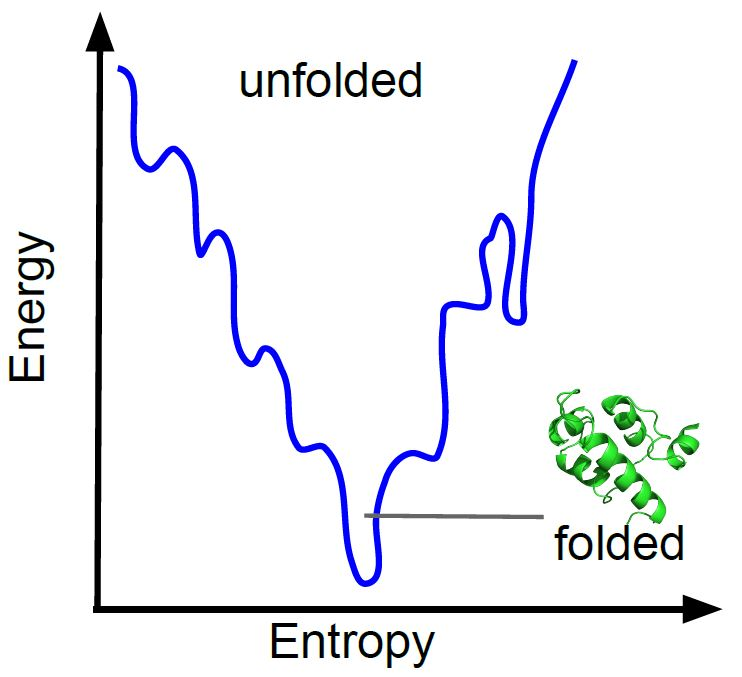
\includegraphics[width=0.4\linewidth]{figures3/folding_funnel.pdf}
  \caption{Protein folding funnel.}
  \label{fig:funnel}
\end{figure}



